\chapter{Exemple d'utilisation}

Les images suivantes représentent un premier aperçu de l'interface graphique de l'application. Nous imaginons donc un scénario d'utilisation qui montre le déroulement d'un usage typique.

\begin{figure}
  \begin{minipage}[t]{8cm}
    \centering
    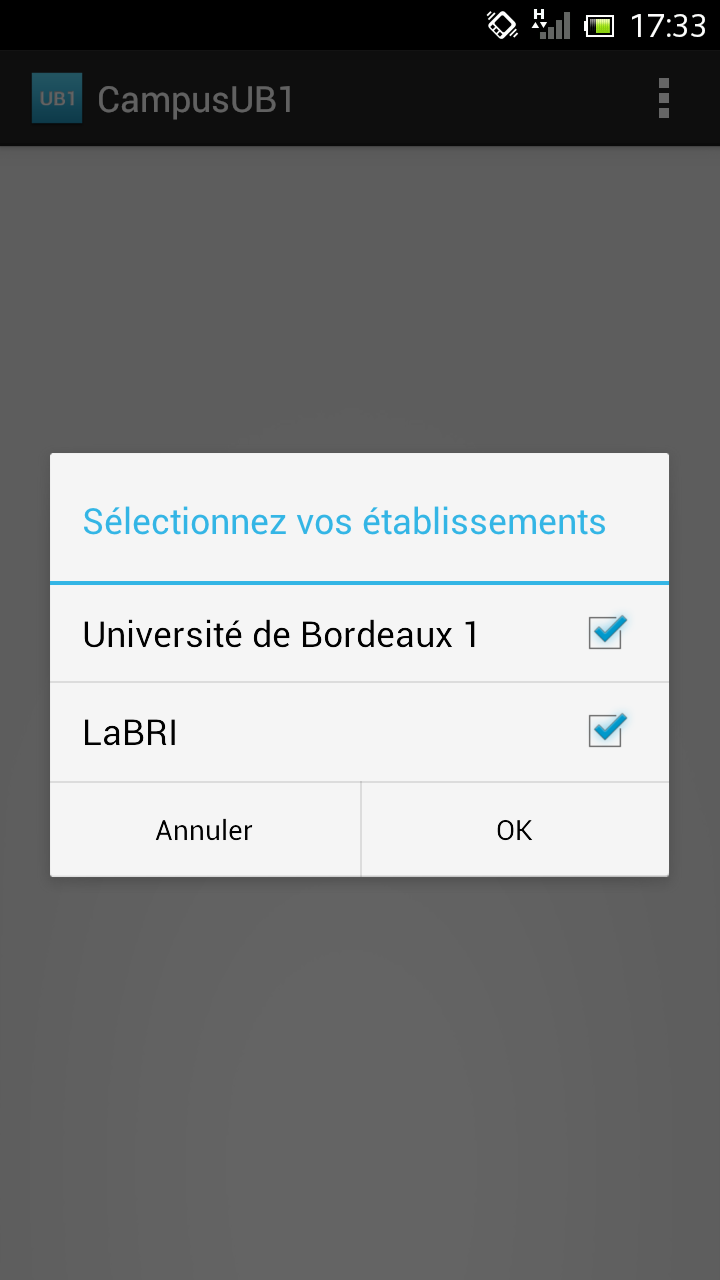
\includegraphics[width=0.8\textwidth]{resources/ui_preview/01}
    \caption{Lors du premier lancement de l'application, l'utilisateur doit sélectionner ses établissements. Une fois ses choix effectués, il sont enregistrés et ne seront plus demandés. Les établissements sont modifiables via les préférences.}
    \label{fig:01}
  \end{minipage}
  \hspace{+20pt}
  \begin{minipage}[t]{8cm}
    \centering
    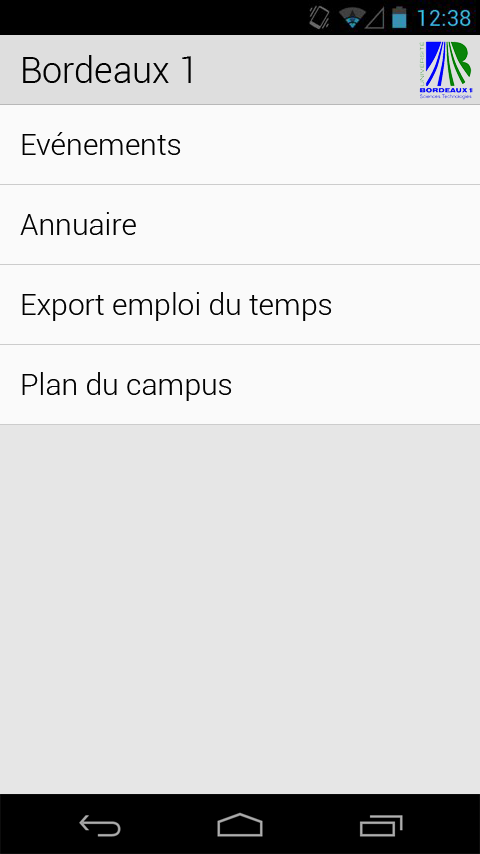
\includegraphics[width=0.8\textwidth]{resources/ui_preview/02}
    \caption{Vue d'accueil de l'application}
    \label{fig:02}
  \end{minipage}
  \hspace{-60pt}
\end{figure}


\begin{figure}
  \begin{minipage}[t]{8cm}
    \centering
    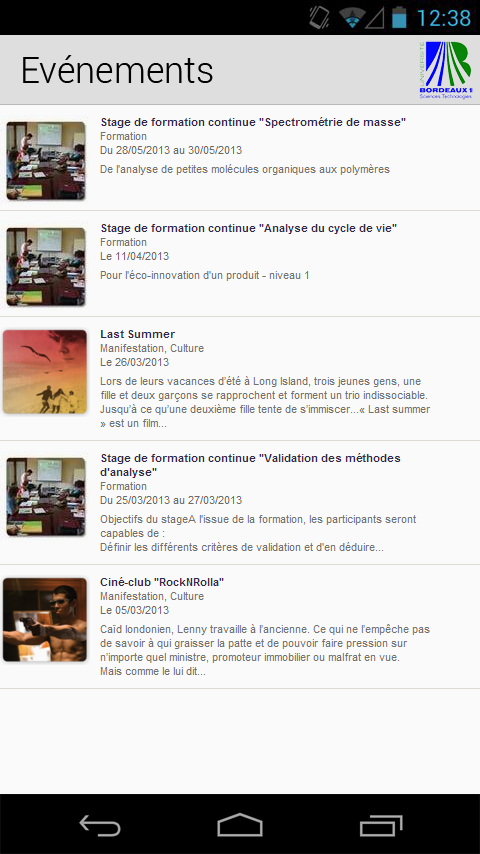
\includegraphics[width=0.8\textwidth]{resources/ui_preview/03}
    \caption{Vue des filtres des résultats en fonction des établissements préalablement choisis. Cette fonctionnalité est accessible via la barre d'action.}
    \label{fig:03}
  \end{minipage}
  \hspace{+20pt}
  \begin{minipage}[t]{8cm}
    \centering
    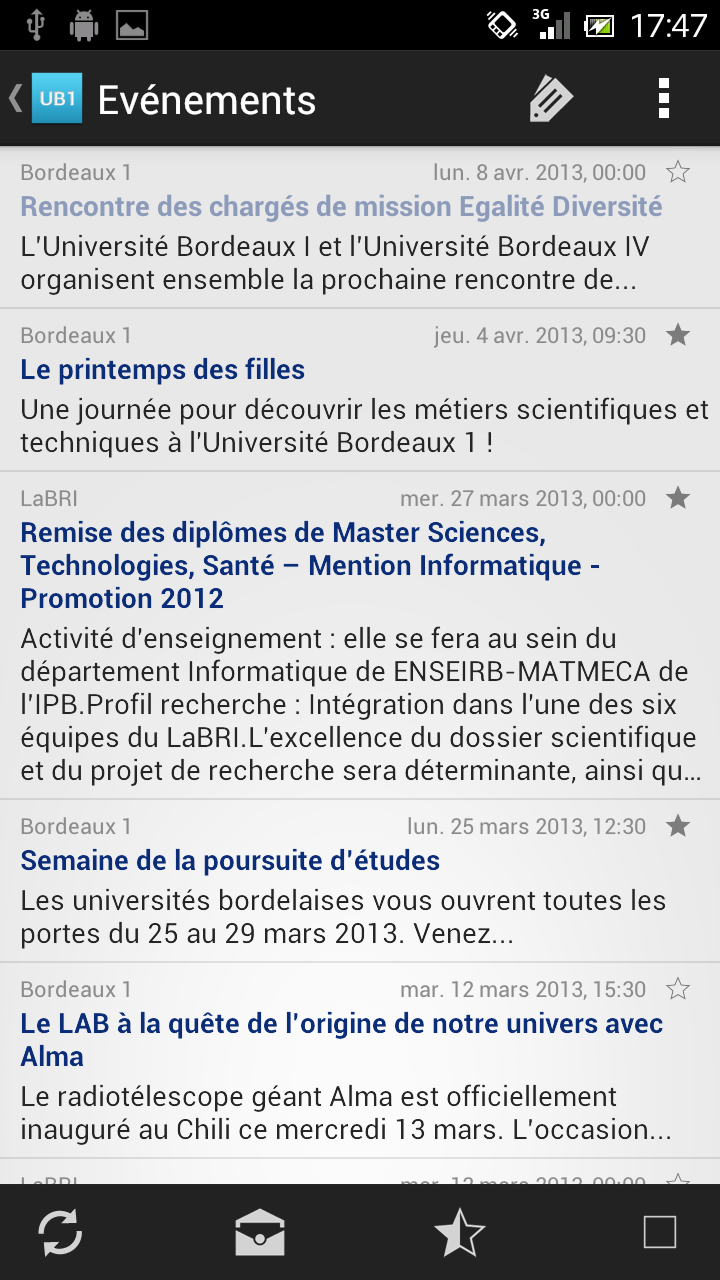
\includegraphics[width=0.8\textwidth]{resources/ui_preview/04}
    \caption{Vue des événements. Pour lire la news et arriver sur l'écran de la figure~\ref{fig:06}, il suffit d'appuyer sur la news correspondante.}
    \label{fig:04}
  \end{minipage}
  \hspace{-60pt}
\end{figure}


\begin{figure}
  \begin{minipage}[t]{8cm}
    \centering
    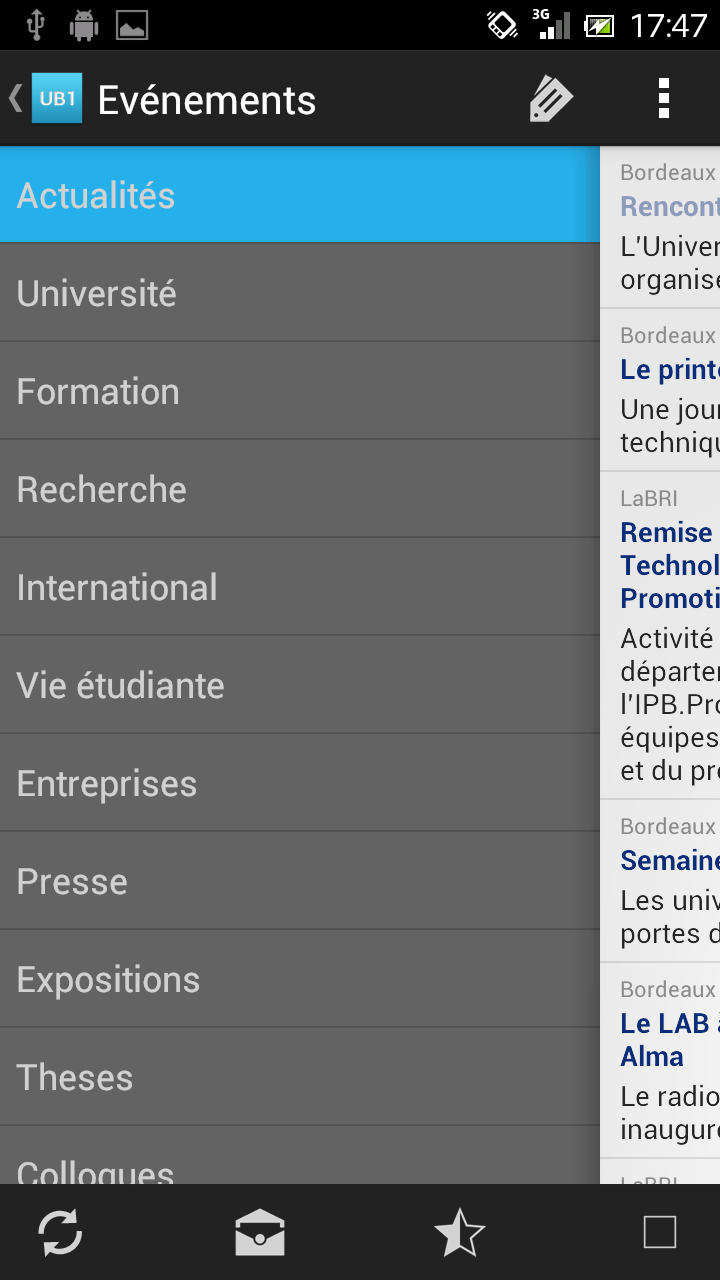
\includegraphics[width=0.8\textwidth]{resources/ui_preview/05}
    \caption{Liste des catégories des news.}
    \label{fig:05}
  \end{minipage}
  \hspace{+20pt}
  \begin{minipage}[t]{8cm}
    \centering
    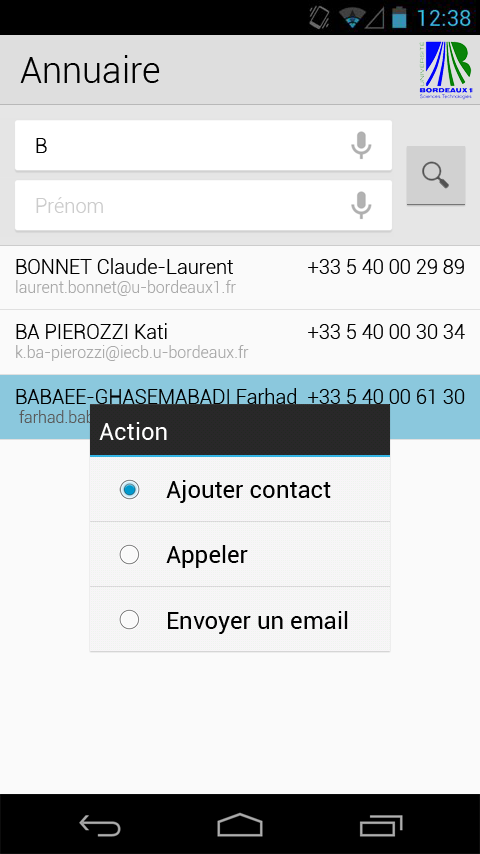
\includegraphics[width=0.8\textwidth]{resources/ui_preview/06}
    \caption{Vue détaillée d'une news. L'icone \emph{Ajouter} de la barre d'action permet d'ajouter l’événement au calendrier du smartphone.}
    \label{fig:06}
  \end{minipage}
  \hspace{-60pt}
\end{figure}


\begin{figure}
  \begin{minipage}[t]{8cm}
    \centering
    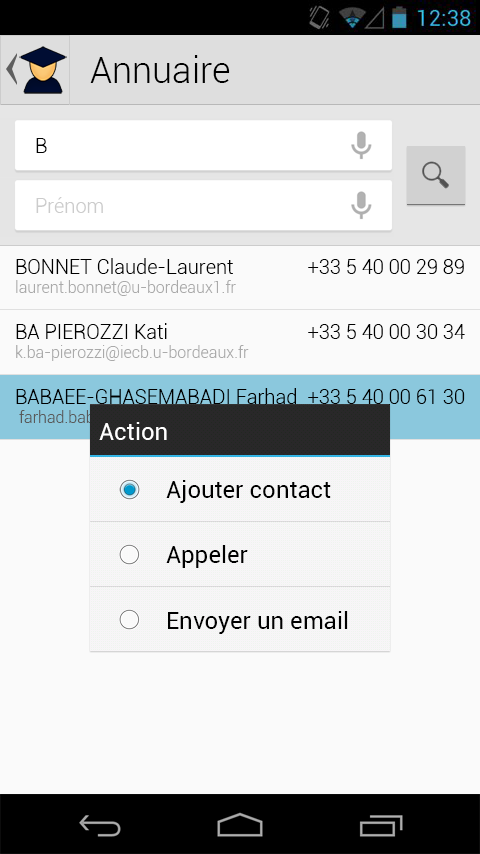
\includegraphics[width=0.8\textwidth]{resources/ui_preview/07}
    \caption{Vue de l'annuaire.}
    \label{fig:07}
  \end{minipage}
  \hspace{+20pt}
  \begin{minipage}[t]{8cm}
    \centering
    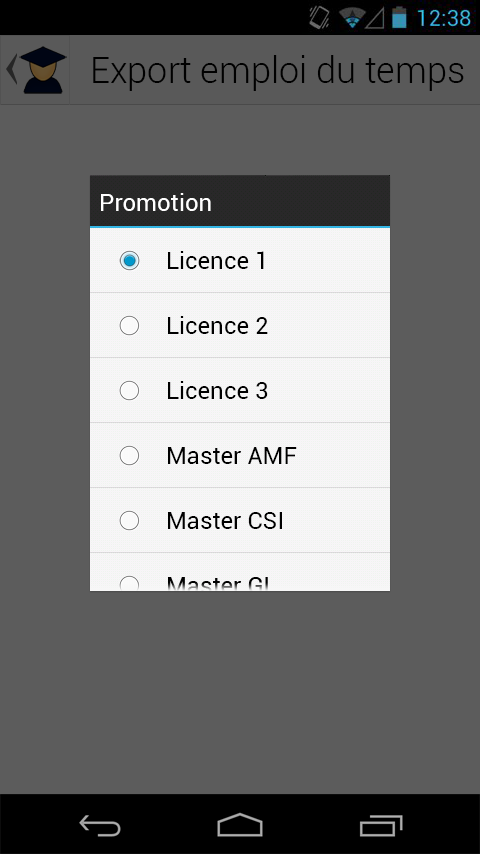
\includegraphics[width=0.8\textwidth]{resources/ui_preview/08}
    \caption{Vue des résultats de l'annuaire.}
    \label{fig:08}
  \end{minipage}
  \hspace{-60pt}
\end{figure}


\begin{figure}
  \begin{minipage}[t]{8cm}
    \centering
    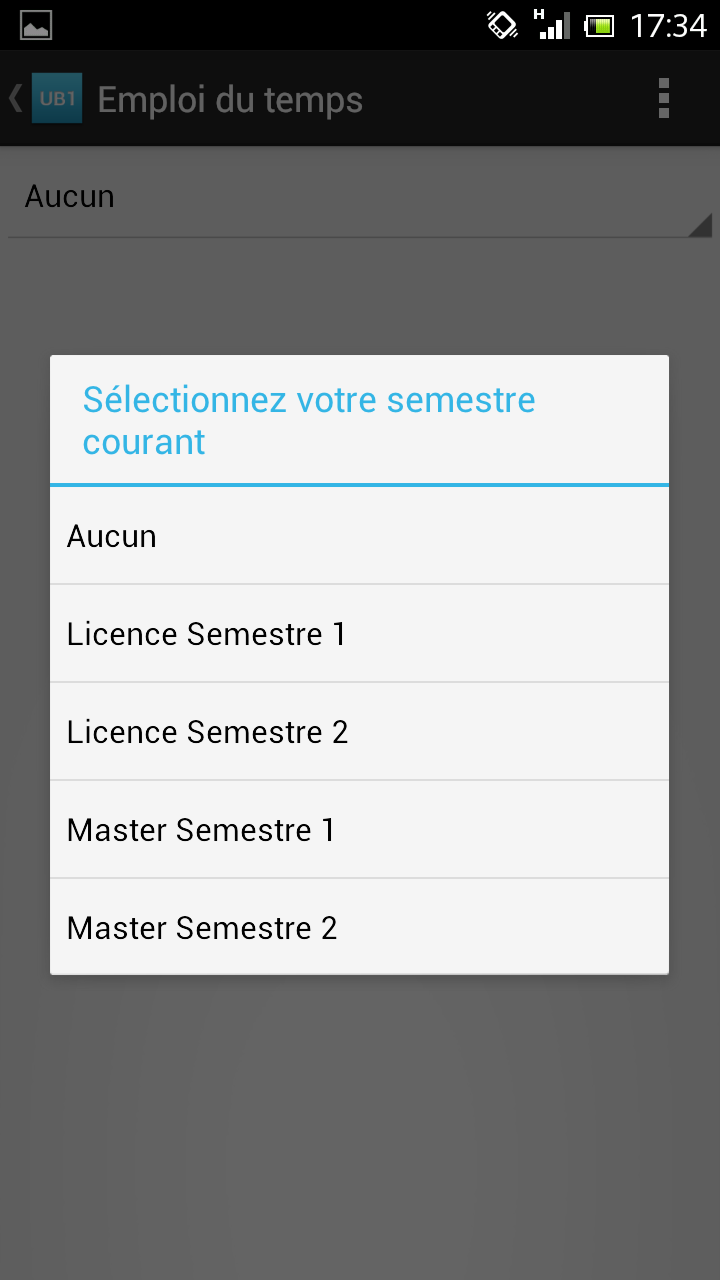
\includegraphics[width=0.8\textwidth]{resources/ui_preview/09}
    \caption{Sélection du semestre de l'emploi du temps.}
    \label{fig:09}
  \end{minipage}
  \hspace{+20pt}
  \begin{minipage}[t]{8cm}
    \centering
    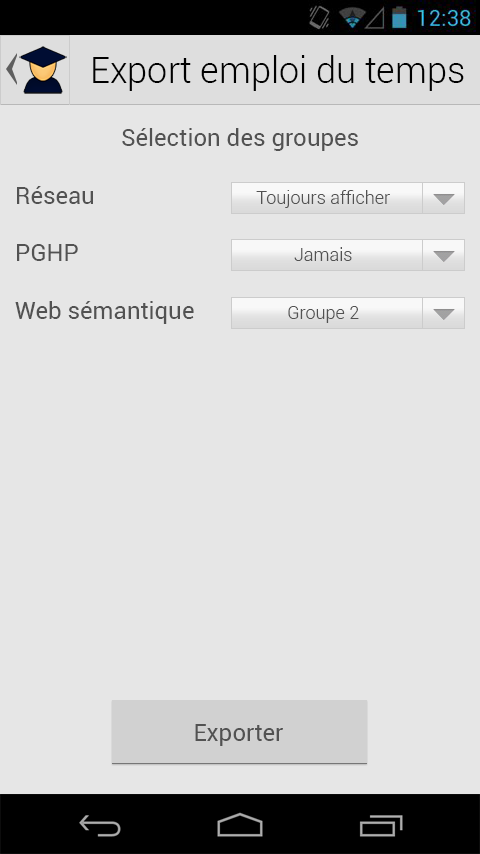
\includegraphics[width=0.8\textwidth]{resources/ui_preview/10}
    \caption{Visualisations possibles de l'emploi du temps.}
    \label{fig:10}
  \end{minipage}
  \hspace{-60pt}
\end{figure}